\section{Related Work}
\label{sec:related}

\begin{figure*}[t]
\centering
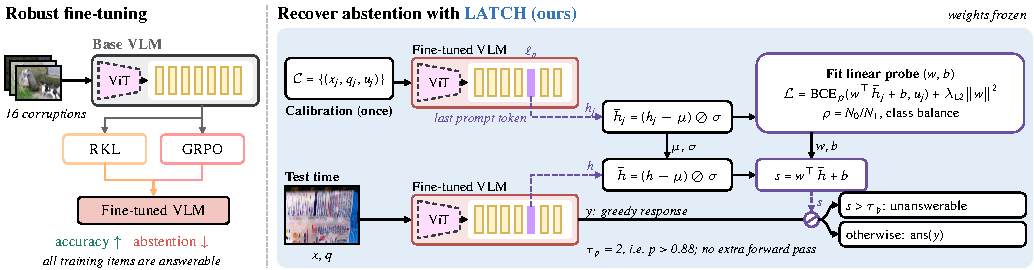
\includegraphics[width=\textwidth]{figures/method.pdf}
\caption{\textbf{Overview.} Robust fine-tuning (RKL or GRPO) raises accuracy but lowers
abstention. LATCH restores it with frozen weights: a latent check, fitted once per model on
a calibration set $\mathcal{C}$, replaces the answer by ``unanswerable'' when the probe
logit $s$ exceeds $\tau_{\mathrm{p}}$ ($P(\text{unanswerable}) > 0.88$). $(x, q)$: image and
question; $y$: response; $u$: answerability label ($u = 1$: unanswerable);
$\mathrm{BCE}_\rho$: binary cross-entropy that weights the $N_1$ unanswerable calibration
items by $\rho = N_0/N_1$, with $N_0$ answerable items. The two baselines are drawn in \cref{fig:supp_retrain,fig:supp_steer}.}
\label{fig:method}
\end{figure*}

\paragraph{Visual understanding.}
Instruction-tuned VLMs built on strong language backbones are now the default interface
for image understanding~\cite{qwen3vl2025,wang2025internvl35,gemmateam2025gemma3technicalreport}.
They are measured on VQA benchmarks targeting compositional reasoning
(GQA~\cite{hudson2019gqa}), language-prior control (VQAv2~\cite{goyal2017vqav2}), and
scene-text reading (TextVQA~\cite{singh2019textvqa}). VizWiz~\cite{gurari2018vizwiz} is
unique for our purpose: its images are taken by blind users, are frequently unreadable,
and a large share of its questions cannot be answered, making it the natural testbed for
abstention under real-world degradation. We use these benchmarks differently from the
accuracy-only protocol they are usually reported with: every accuracy number is paired
with an abstention measurement, refusals on VizWiz's unanswerable questions and on copies
of the other three benchmarks with the image withheld, because accuracy alone hides the
regression we study.


\paragraph{Corruption-robust post-training.}
ImageNet-C~\cite{hendrycks2019imagenetc} established common corruptions (noise, blur,
weather and digital artifacts at graded severity) as the standard robustness benchmark,
and Usama~\etal~\cite{usama2025analysing} showed that VLM accuracy on TextVQA and GQA drops
substantially under them. Recent work trains VLMs to close this
gap~\cite{he2026videoreasoningmodelsready,tang2026robustr1,liu2026roma}, building on two
post-training recipes. Distillation transfers a teacher's behavior to a
student~\cite{hinton2015distilling,kim2016sequence}; for generative models, reverse-KL
and on-policy variants work best~\cite{gu2024minillm,agarwal2024onpolicydistillationlanguagemodels},
and we combine both with a clean-image teacher and a corrupted-image student
(\cref{sec:method-ft}). GRPO~\cite{shao2024deepseekmath} replaces PPO's value
network~\cite{schulman2017ppo} with group-relative advantages and has become a standard
recipe for fine-tuning with verifiable rewards~\cite{guo2025deepseekr1,liu2025visualrft}.
We follow the corrupted-VQA protocol of~\cite{usama2025analysing} but train with a
different corruption engine, so $11$ of the $19$ evaluation corruptions are never seen in
training. Neither recipe is free of side effects. Fine-tuning erodes capabilities it never
targets, from safety alignment~\cite{qi2024finetuning} to previously learned
skills~\cite{kirkpatrick2017overcoming,luo2023empirical,zhai2024forgetting}, and
reinforcement fine-tuning reduces refusals on unanswerable questions in language
models~\cite{song2025hallucinationtax}. Robust post-training, however, is evaluated on
accuracy alone. We show that it silently erodes visual abstention, and that GRPO does so
through an \emph{always-answer} shortcut that arises because its reward is defined only
over answerable inputs.

\paragraph{Visual abstention and the representation--output gap.}
Knowing when not to answer is central to
reliability~\cite{geifman2017selective,kirichenko2025abstentionbench}, and VLMs readily
answer questions that the image cannot support. Several benchmarks measure this failure
directly~\cite{miyai2024upd,zhu2025mohobench,saadat2025visiontrap,madhusudhan2026knowing,
chandu2025certainly}, and lightweight methods add abstention to a fixed model, either by
estimating answer reliability~\cite{khan2024consistency,srinivasan2024recoverr} or by
attaching an unanswerability head~\cite{vardi2025clipup}. Closest to us, two concurrent
works find that VLMs know more than they say: linear probes decode answerability from
hidden states even when the final answer ignores it, in physical-reasoning
videos~\cite{pramono2026trapsbench} and in static images~\cite{he2026knowing}, where
Rep2Act closes the gap by fine-tuning. All of this work studies a \emph{fixed} model. We
show that the gap moves: corruption-robust post-training widens it, at the reasoning step
for distillation and at the answer step for GRPO. Like CLIP-UP, LATCH adds a
light classifier and leaves the backbone untouched, but it reads each fine-tuned model's
own hidden states and, unlike Rep2Act, changes no weights.

\paragraph{Activation steering.}
Steering methods edit a model's internal activations at inference time to change its
behavior~\cite{turner2023actadd,li2023iti,zou2023repe}. Contrastive Activation
Addition~\cite{rimsky2024caa} adds the mean activation difference between contrasting
examples during generation, and refusal in particular is often controlled by a single such
direction~\cite{arditi2024refusal}. We use contrastive steering as a baseline, with
directions built from base-versus-fine-tuned responses that push the fine-tuned model back
toward the base model's abstention.
